%" vim: fdm=marker:fen:fdl=0
% Manufacturing of Planar Detectors Chapter intro%{{{
\chapter{Manufacturing of Planar Detectors}
The manufacturing process of a planar HPGe detector begins with a slice from a crystal boule that has been tested for quality and is know to be detector grade.
Typical boules slices are solid discs that can range from a few millimeters up to several centimeters in thickness and 5+ centimeters in diameter.
This large size allows for several detector samples to be cut from each slice so careful geometry considerations are important in order to minimize wasted material.
The goal is for the detector sample to look approximately like figure \ref{fig:dummydet} which is an example of a planar detector with so called top hat geometry.
\begin{figure}[htpb]
\centering
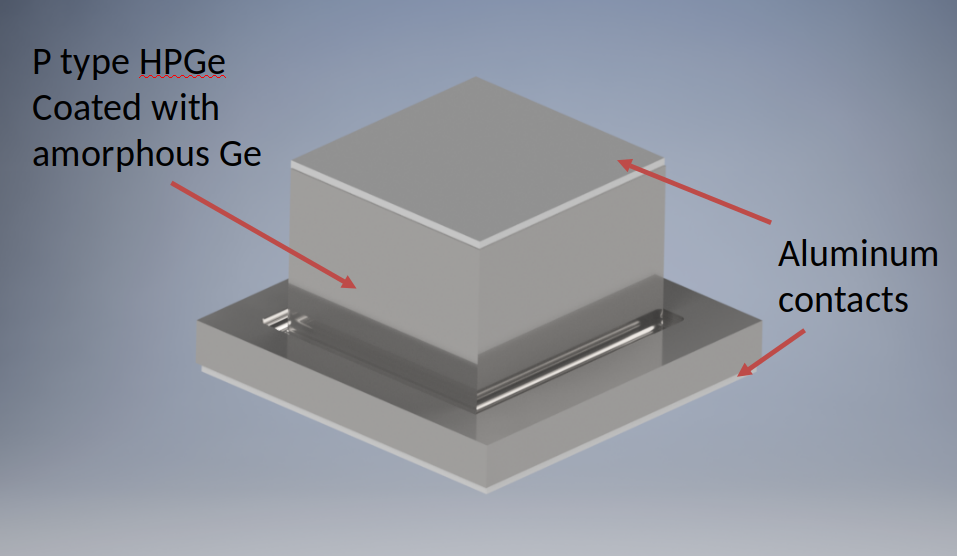
\includegraphics[width=0.5\textwidth]{dummy-det}
\caption{Example detector geometry with four wings}
\label{fig:dummydet}
\end{figure}
The brims of the hat are called wings and serve as a dead area of the detector for handling during the manufacturing process.
The detector is not required to be perfectly square to work so length and width can vary within a few centimeters.
What is of importance are the overall thickness and that the top and bottom faces are parallel.
Due to the relatively long mean free path of gamma rays in germanium, a detector should aim to be at least one centimeter thick.

Once considerations for geometry have been made, the detector manufacturing process begins.
To start, the germanium boule slice is cut into several rectangular cubes.
Then, work proceeds using one of the cubes, saving the rest for the next time.%}}}
% Section: Mechanical Processing%{{{
\section{Mechanical Processing}
The diamond saw under discussion is the SYJ-400 Precision CNC Dicing/Cutting Saw from Shenyang Kejing Auto-Instrument Co.
The structure of this diamond saw is shown below in Figure \ref{fig:diamondsaw}.
It is operated using a CNC controller with setting for the cutting speed, length, time, depth, lifting height, rest time, and movement speed.
All of these parameters are edited using the attached CNC controller. 
There are four separate screens with adjustable parameters that are shown with translations in Figure \ref{fig:control-screen}. 
Each of these parameters are in millimeters or millimeters per minute depending on the operation.
\begin{figure}[htpb]
\centering
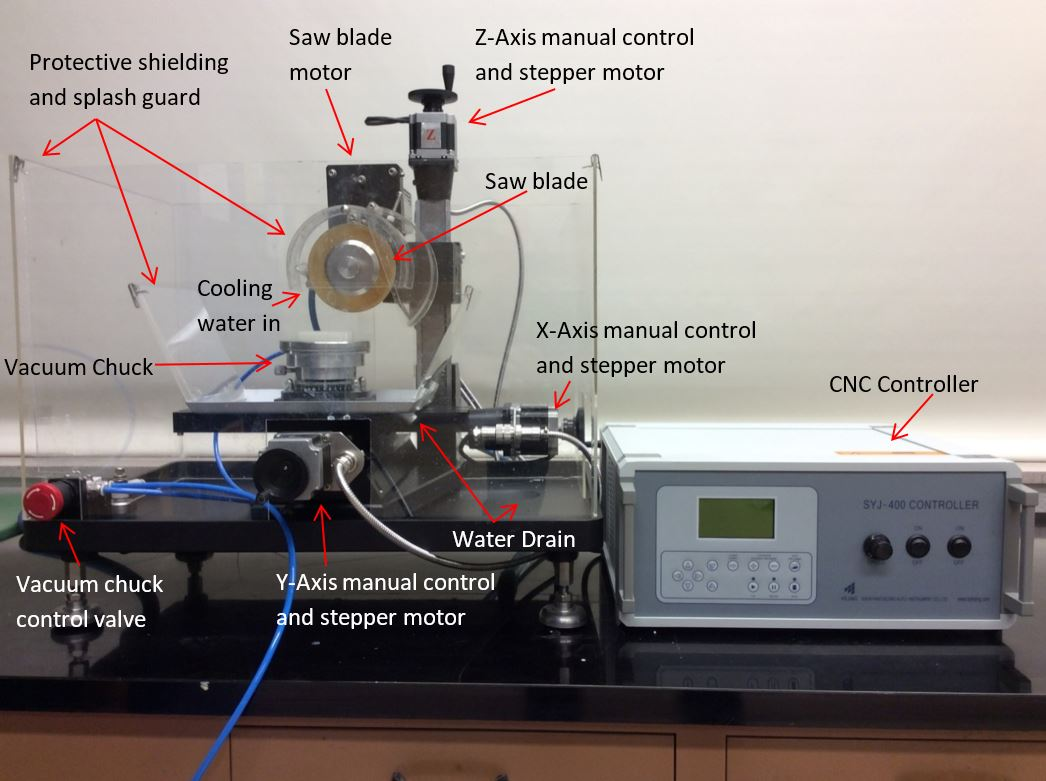
\includegraphics[width=0.5\textwidth]{diamond-saw.jpg}
\caption{The diamond saw used to cut boules into detector samples.}
\label{fig:diamondsaw}
\end{figure}

\begin{sidewaysfigure}
\includegraphics[width=\textwidth]{control-screen}
\caption{These are the four settings screens and translations from the diamond saw controller.}
\label{fig:control-screen}
\end{sidewaysfigure}

Before turning on the power to the diamond saw, it is important to take care of all of the necessary adjustments such as changing blades and placing the sample onto the vacuum chuck.
It is important to do this before supplying power in order to prevent the saw from somehow starting itself.
To switch blades, first remove the finger screw, labeled 1, on the outside of the splash guard covering the blade. Then remove the finger screw, labeled 2, that holds the blade clamps.
Remove the outer blade clamp and the blade can be switched out.
Depending on the blade size, it may be necessary to change to a larger splash guard.
To do this, first remove finger screw 1 on the outside of the splash guard, then remove the two hex screws, labeled H, on the back plate.
It might be necessary to remove the blade to access these screws.
You can then install the new splash guard and blade working in the opposite order to put everything back together.
\begin{figure}[htpb]
\centering
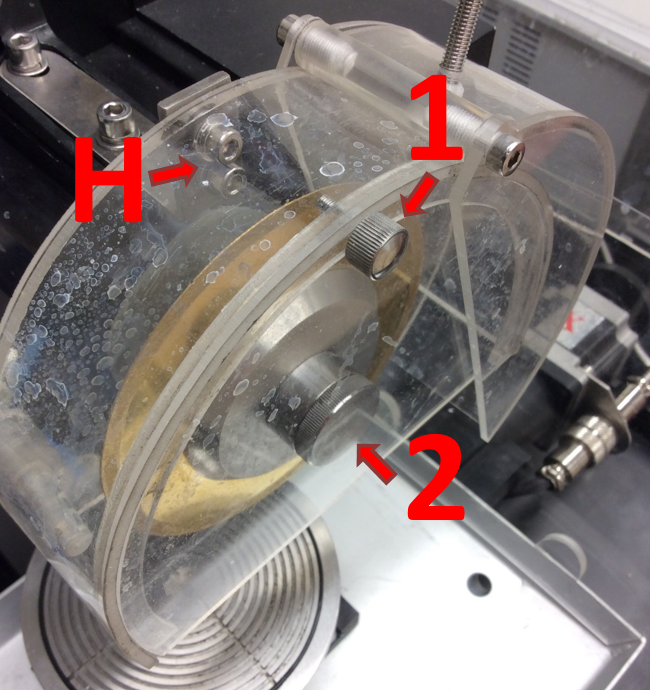
\includegraphics[width=0.5\textwidth]{blade-case}
\caption{This is the blade and shielding on the diamond saw.}
\label{fig:blade-case}
\end{figure}

There are currently three different blades available for cutting.
They include: 4” electroplated diamond blade, 4” full sintered diamond blade, and a 4” grinding blade. 
\begin{figure}[htpb]
\centering
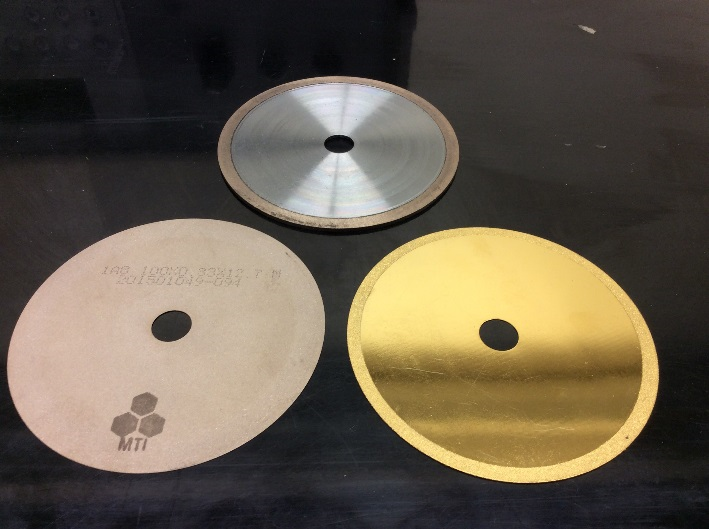
\includegraphics[width=0.5\textwidth]{blades}
\caption{Three different blade types for cutting germanium.}
\label{fig:blades}
\end{figure}

The next step is to mount your sample onto the vacuum chuck.
It is essential to do this before powering on the diamond saw to avoid accidents.
Place the steel sample holder onto the vacuum chuck and adjust it so it is properly aligned.
Powering on the vacuum will come in the next steps.
\begin{figure}[htpb]
\centering
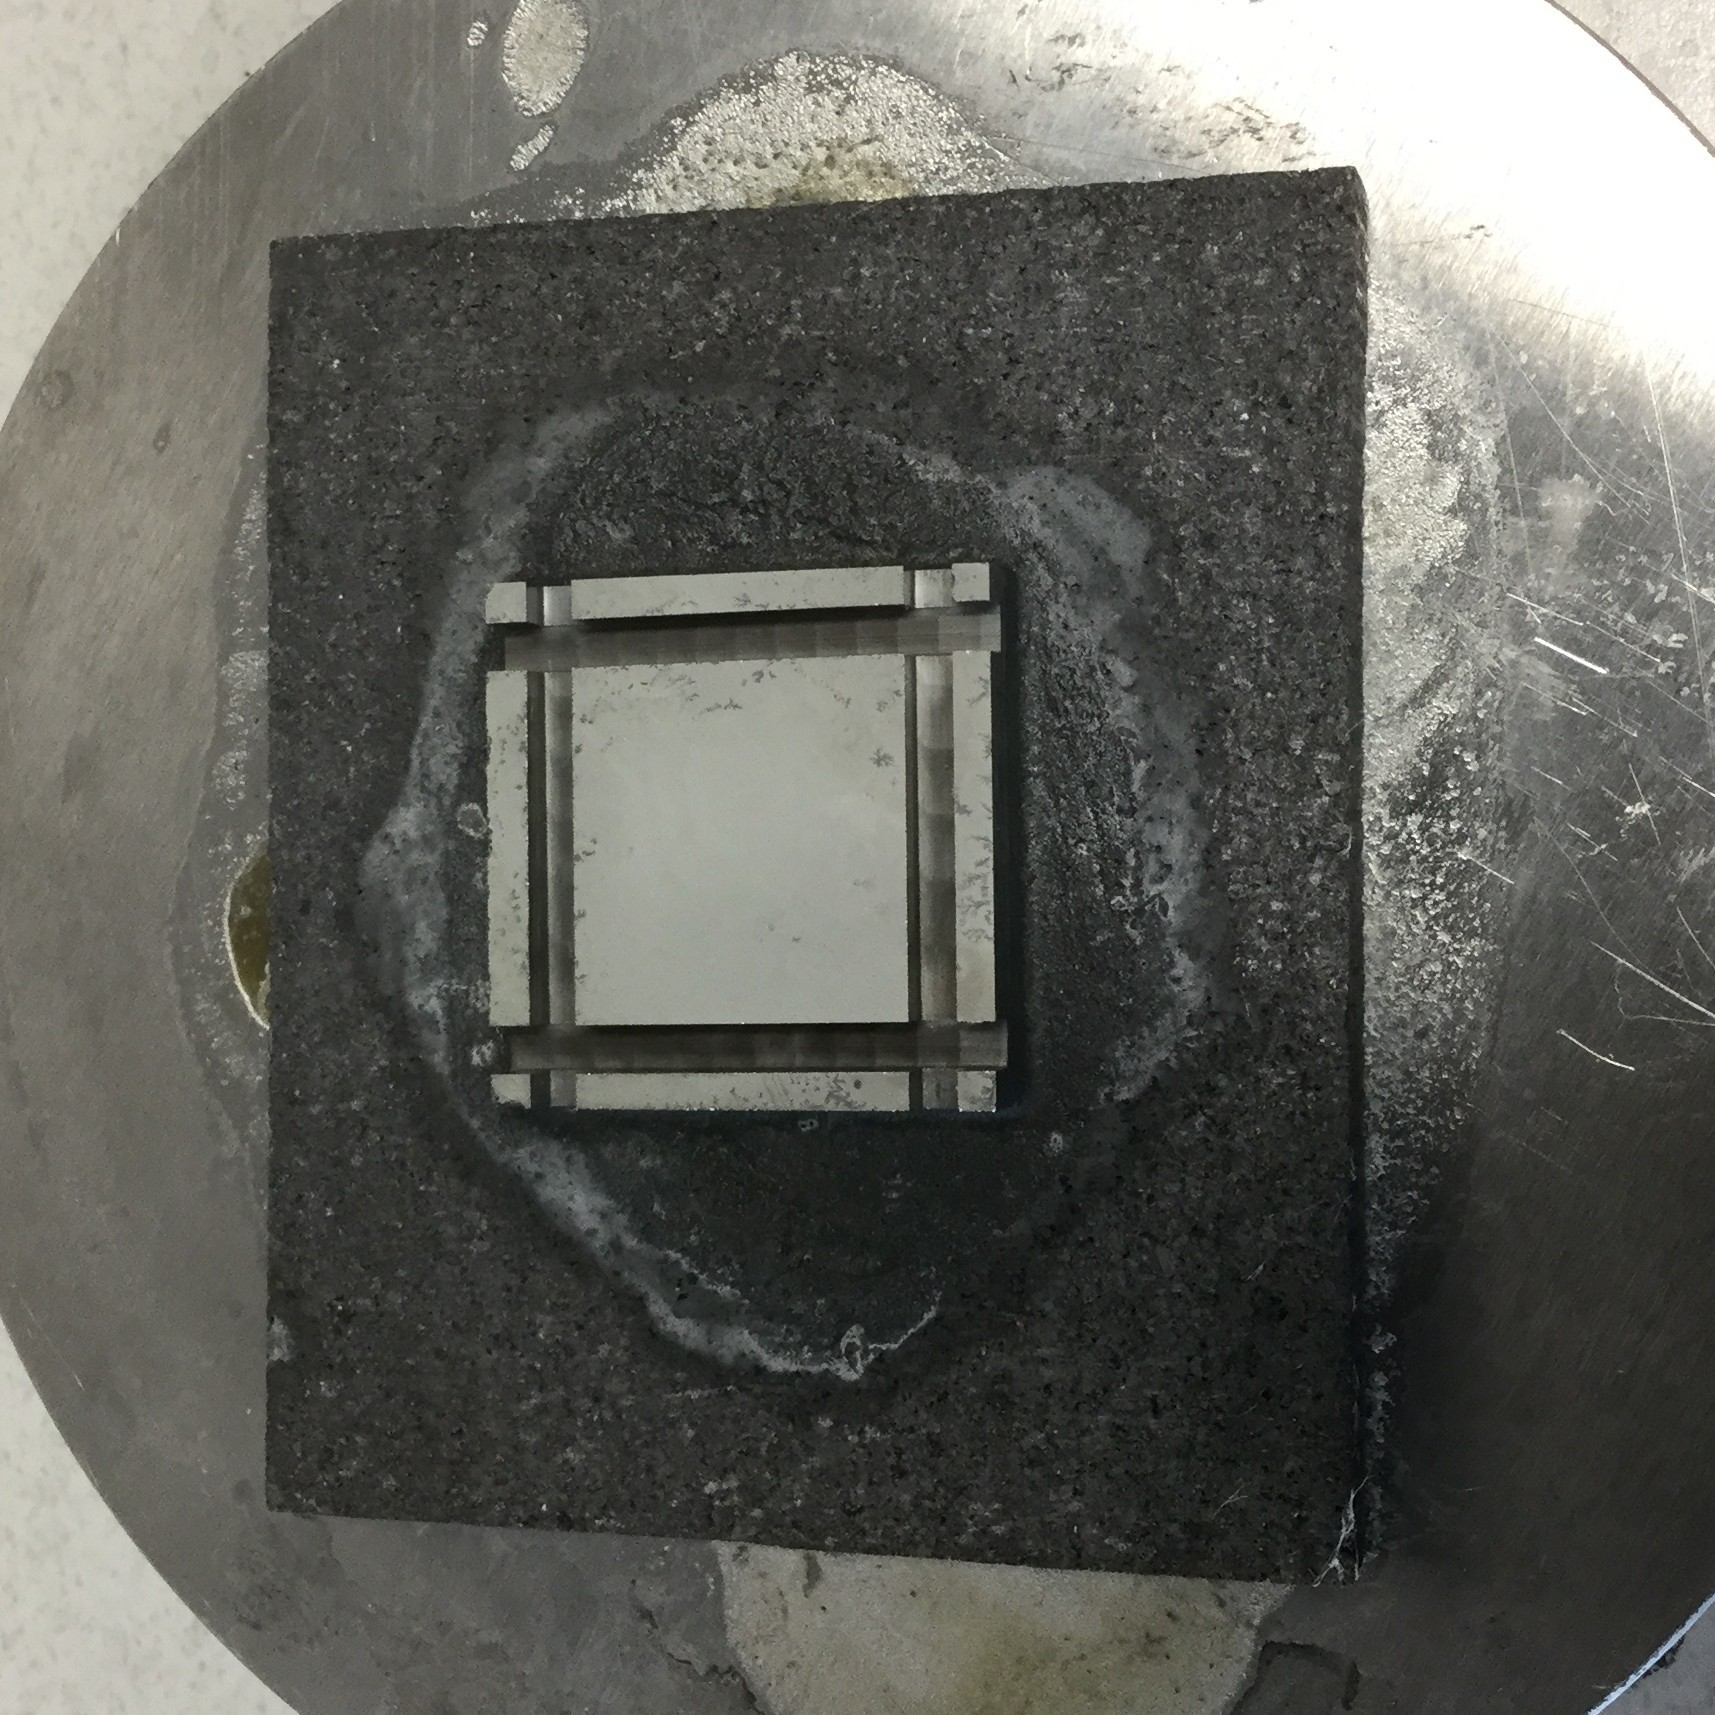
\includegraphics[width=0.5\textwidth]{cut-sample}
\caption{A germanium sample mounted on graphite which is then mounted on a stainless steel chuck.}
\label{fig:cut-sample}
\end{figure}

To start the diamond saw, first turn on the power strip.
This will provide power to the vacuum pump and the up/down power converter.
The next step is to power on the up/down converter that is located under the table that supports the diamond saw.
This will provide a stepped up voltage to the CNC controller (which powers the saw) and the water pump.
\begin{figure}[htpb]
\centering
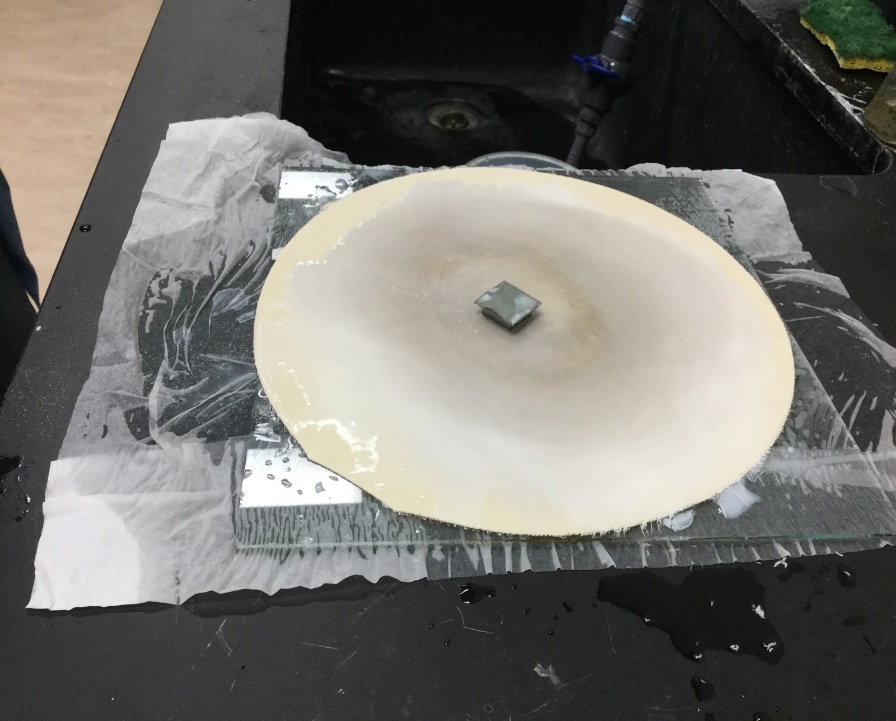
\includegraphics[width=0.5\textwidth]{lapping.jpg}
\caption{An example of lapping the detector sample}
\label{fig:lapping}
\end{figure}%}}}
% Section: Chemical Processing%{{{
\section{Chemical Processing}

\begin{figure}[htpb]
\centering
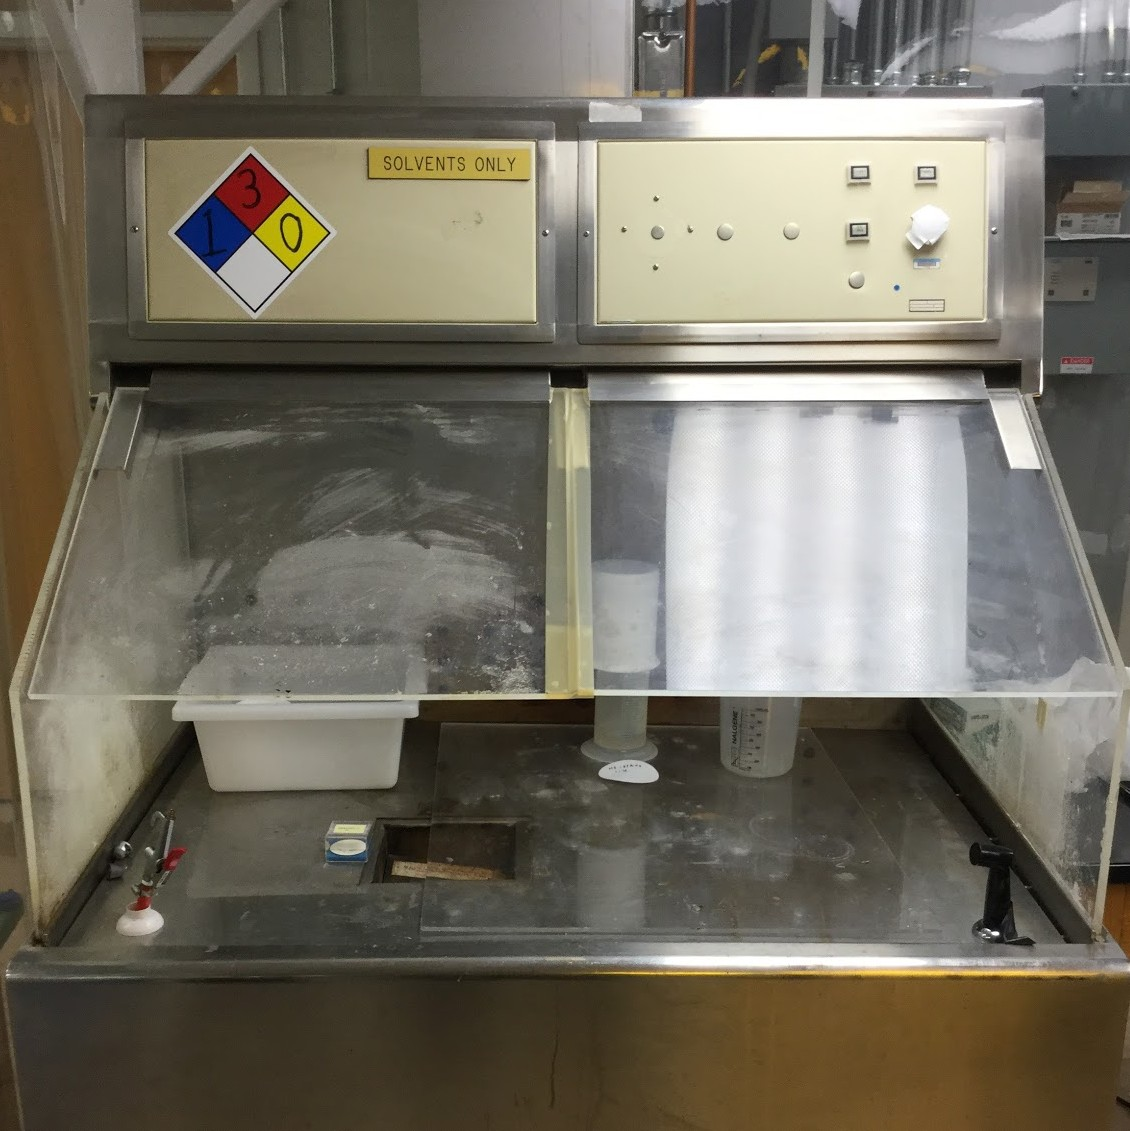
\includegraphics[width=0.5\textwidth]{metal-hood.jpg}
\caption{Metal hood for use with solvents}
\label{fig:metalhood}
\end{figure}


\begin{figure}[htpb]
\centering
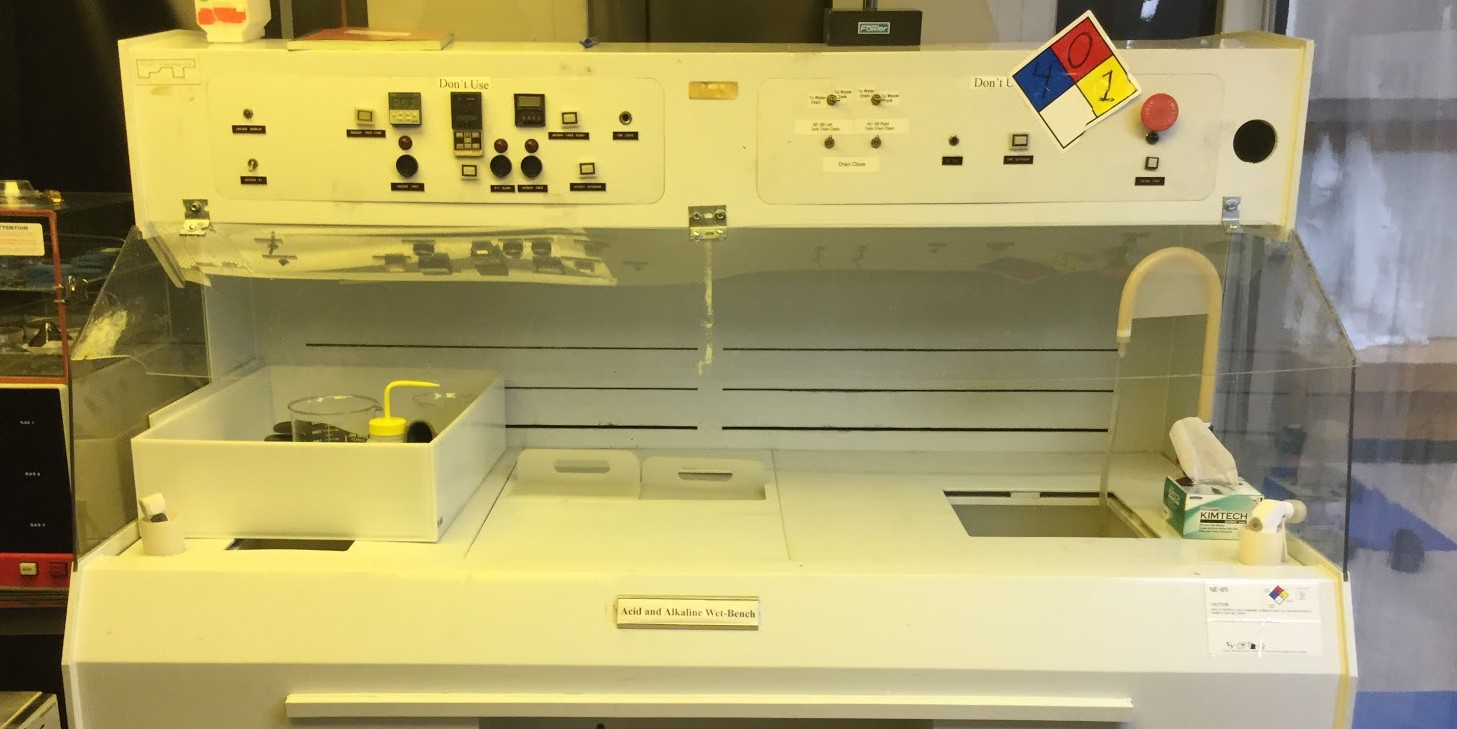
\includegraphics[width=0.5\textwidth]{plastic-hood.jpg}
\caption{Plastic hood for use with acids.}
\label{fig:plastichood}
\end{figure}

%}}}
% Section : Amorphous Ge Deposition%{{{
\section{Amorphous Ge Deposition}

Need information on the working principles of sputtering machine
also need more on the range measurement, marks papers citing specific values for settings 
\subsection{Principles of Sputtering}

\subsection{Operating Procedure}
The sputtering machine at USD is a Perkin-Elmer 4400 Sputtering System.

The operating procedure for the sputtering machine is complex and care is required to make sure the system maintains working order.
It is a complex system with multiple valves, controls, power supplies, vacuum systems, and pressure monitors that all work in conjunction to deposit a thin layer of amorphous germanium on the detector sample.
One key component of the system is a cryopump that uses pressurized helium gas to quickly vacuum the system to the proper pressure.
The cryopump system can be seen in Figure ~\ref{fig:sput-flow} as blue boxes with labels connected by green lines.
The green lines exchange the helium between the cold head connected to the vacuum chamber and the compressor located in the pump room.
Before the sputtering procedure can begin, the cryopump must be turned on to allow the cold head to cool from room temperature to approximately 20K.
Prior to cooling down the cryopump, it must be vacuumed to below 100 mtorr using the rough pump describe later.
In order to vacuum the cryopump, open the forline valve shown as E in ~\ref{fig:sput-flow}; close the valve before turning on the cryopump.
The on/off switch for the compressor is located on the panel with the other valve toggles and is labeled as "HY-VAC PUMP"

Once the cryopump is cooled down to the proper temperature, the sputtering procedure can begin.
As seen in Figure ~\ref{fig:sput-flow}, there are multiple valves for opening and closing various gas and vacuum lines.
These valves are all pneumatically opened and closed so they require a constant supply of pressurized air at 60 psi.
This pressurized air is supplied by a large Kaeser SX 5 compressor located in the pump room and shown in Figure ~\ref{fig:comp-air}.
\begin{figure}[htpb]
\centering
\includegraphics[width=\textwidth]{comp-air}
\caption{Kaeser SX 5 compressor}
\label{fig:comp-air}
\end{figure}
The compressor is turned on or off by pressing the green or red button on the control interface shown on the top left side of the figure.
Once turned on, it will automatically increase in pressure until it reaches a set point around 100 psi.
The pressure out is then reduced or increased by adjusting the pressure regulator shown on the bottom left.
It is important to check the pressure often to make sure that it is sufficiently high for if it drops too low, valves will return to the default closed position.

Once the system has been supplied with pressurized air, the valves can be opened or closed and the system is ready to be operated.
The next step is to load the detector sample into the sputtering machine and prepare for deposition.
The sputtering system should always be kept under vacuum so before it can be opened it must be returned to standard atmospheric pressure.
This is done by opening the vent valve and filling the chamber with dry nitrogen.
The toggle switch for the vent valve is located at 'A' in Figure ~\ref{fig:sput-flow}.
The nitrogen in routed in from a tank located in a separate room behind the pump room and is kept at approximately 10 to 15 psi.

After the chamber has returned to atmospheric pressure it can be opened using a hydraulic lift system that is powered through the RF power generator.
The sample can now be carefully placed inside the chamber centering it under the amorphous germanium target as seen in Figure ~\ref{fig:sput-open}.
\begin{figure}[htpb]
\centering
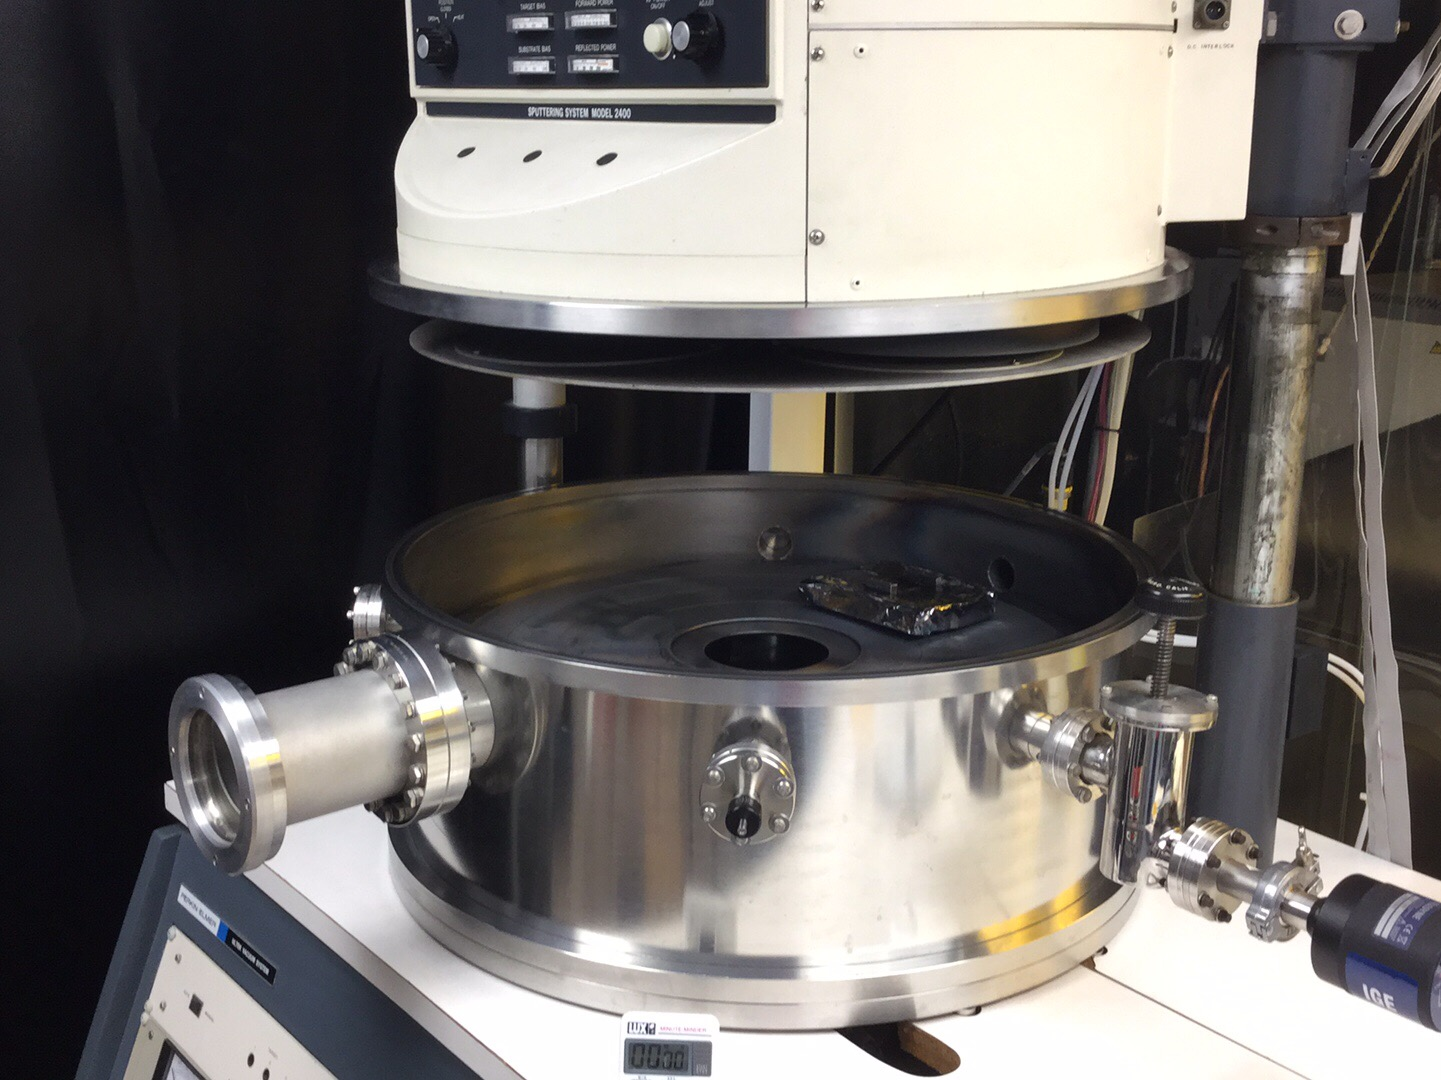
\includegraphics[width=0.6\textwidth]{sput-open.JPG}
\caption{Sputtering machine with chamber open}
\label{fig:sput-open}
\end{figure}
A jig is used to hold the detectors by the wings during the sputtering process.
It is designed to be adjustable, allowing for various detector sizes and geometries.
After the detector sample has been chemically etched it can be loaded onto the jig and then into the sputtering machine.

Once the sample is loaded the chamber can be closed and vacuum pumping can begin.
The first stage of pumping is done by a rough pump which takes the chamber from atmospheric pressure down to below 100 millitorr.
The rough pump is turned on or off by switching an electrical breaker located outside of the clean room.
After the pump is on and running normally, the roughing valve can be opened.
Opening the roughing valve allows the rough pump to vacuum the chamber from atmospheric pressure to around 100 mTorr.

Once the chamber has reached some pressure between 50-100 mTorr the roughing valve can be closed and the HY-VAC VALVE, shown as D in Figure \ref{fig:sput-flow}, can be opened.
The cryopump will then be able to vacuum the system to the required $10^{-6}$ Torr for sputtering.
The sputtering machine takes less than five minutes to go from atmosphere to $10^{-3}$ Torr using the rough pump and a further 2-3 hours to reach $10^{-6}$ Torr using the cryopump.

After proper vacuum pressure is achieved the sputtering deposition procedure can start.
The first thing is to start the water chiller and make sure the proper lines are selected.
The chiller is used to provide cooling to the target and stage during deposition as the plasma generates considerable heat.
It is located in the pump room and is show in Figure ~\ref{fig:water-cool}.
The middle picture of the figure shows the side view of the chiller where the separate lines to the sputtering and e-beam machines are visible.
The selection of lines is done by switching two valves on the back of the water chiller.
The handles of the valves indicate the direction of flow and is used to determine which line is selected.
\begin{figure}[htpb]
\centering
\includegraphics[width=\textwidth]{water-cool}
\caption{Water chiller for cooling the sputtering machine and e-beam evaporator}
\label{fig:water-cool}
\end{figure}

Once the water chiller has reached the set point temperature of \SI{10}{\celsius}, the deposition can start.
First the RF power supply should be turned on by flipping the switch at the base of the front.
The throttle valve, shown as C in Figure ~\ref{fig:sput-flow}, can now be turned on to limit the vacuuming of the chamber.
Now the mixed gas can be vented into the chamber using the gas flow adjuster show in the figure.
To the left of the flow controller is the togle switch to open the mixed gas line.
Then, the flow controller is turned on and set to approximately 50 SCCM.
Due to the throlle valve being on, the chamber will begin to increase in pressure based on the flow controller setting.
The key is to adjust the flow rate until a steady 14 mTorr chamber pressure is achieved.

After the chamber has stabalized at 14 mTorr the RF power can be introduced to the gas in order to generate the plasma required for sputtering.
This is done by pressing the power on button at the top of the chamber show in Figure.
The power can then slowly be increased to the marked point.
During this increase in power, the tune and load must be adjusted to keep the reflected power to a minimum and make sure all the power is transfed into the gas.
At a certain point, the plasma will form and the reading for forward and reflected power will jump up.
It is again necessary to quickly readjust the tune and load to get the reflected power back to 0.
After the reflected power is reduced, the power can be further adjusted to the required level, usually around 100 watts.
Once the plasma is generated, the user must wait for at least five minutes with the shutter closed to bombard the target and clean off the outer layer.
After this five minutes 
\begin{sidewaysfigure}
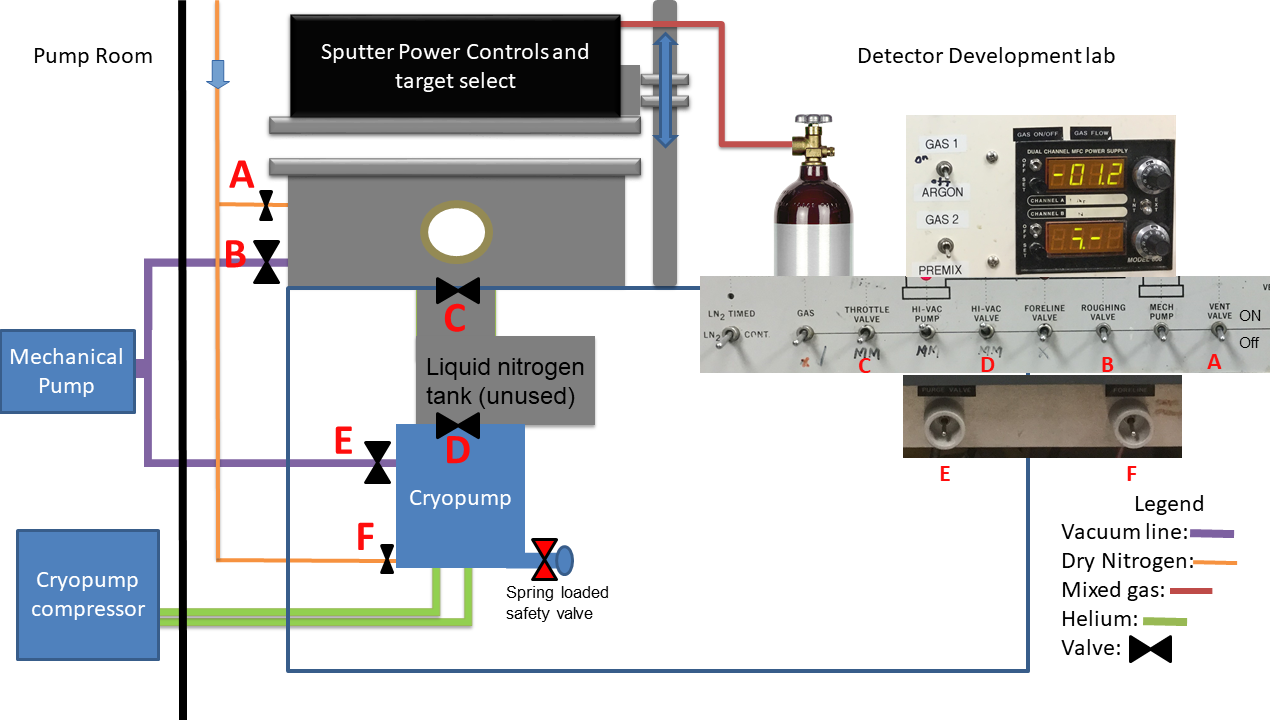
\includegraphics[width=\textwidth]{sput-flow}
\caption{This is a diagram of the Sputtering machine vacuum and gas system. Each valve is connected to a pressurized air line.}
\label{fig:sput-flow}
\end{sidewaysfigure}%}}}
% Section: Aluminum deposition%{{{
\section{Aluminum Deposition}

\begin{sidewaysfigure}
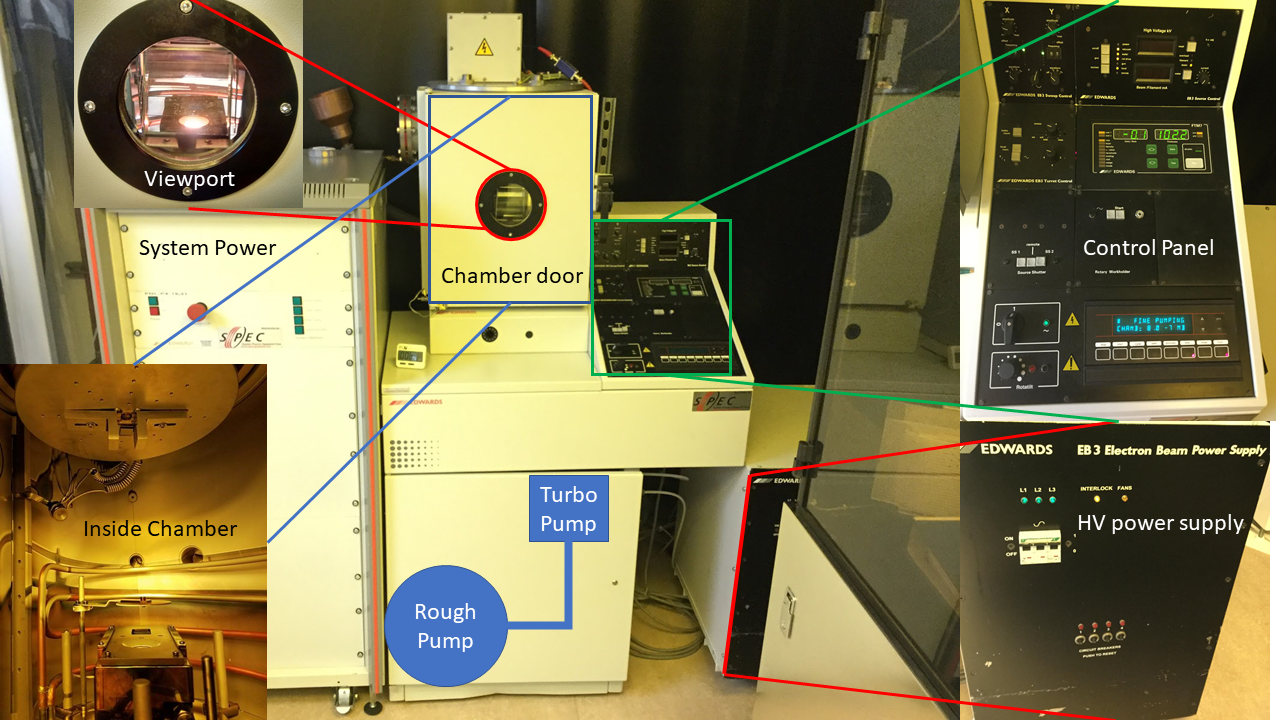
\includegraphics[width=\textwidth]{ebeam-flow}
\caption{This is a diagram of the of the electron beam machine.It is used to deposit aluminum onto the detector sample.}
\label{fig:ebeam-flow}
\end{sidewaysfigure}%}}}
% Section: Final Steps%{{{
\section{Final Steps}%}}}
